\documentclass[tikz, border=10pt]{standalone}
\usepackage{tikz}
\usepackage[sfdefault]{roboto}
\usepackage[T1]{fontenc}
\usetikzlibrary{shapes.misc, positioning, arrows.meta, fit, calc, backgrounds}

\begin{document}

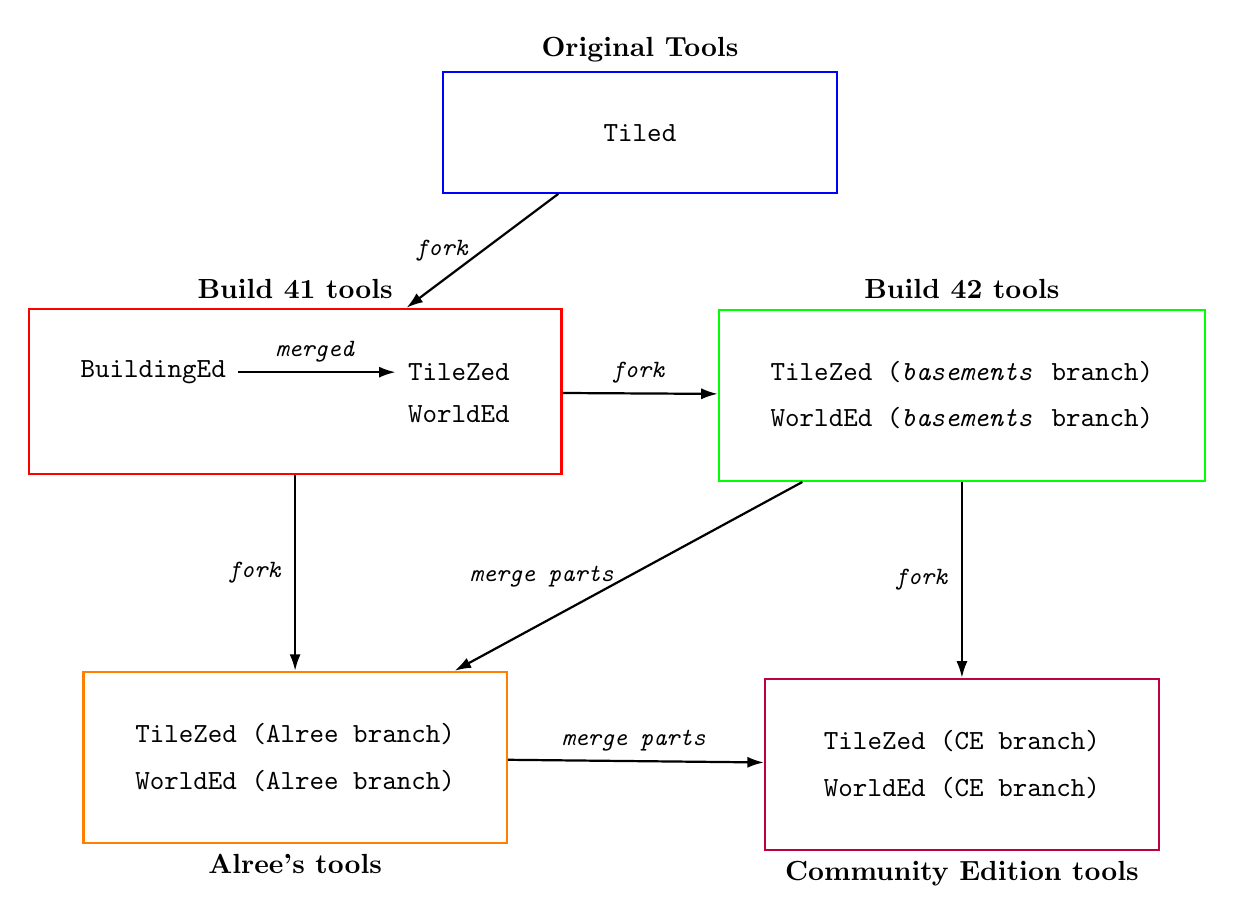
\begin{tikzpicture}[
    node distance=0.3cm,
    box/.style={rectangle, draw, thick, minimum width=5cm, inner sep=0.5cm},
    func/.style={font=\ttfamily, inner sep=0.15cm},
    arrow/.style={-{Latex[length=6pt, width=4pt]}, thick},
    line/.style={thick},
]

%% NODES
    % original tools
    \node[func] (ext_tileed) {Tiled};
    \node[box, draw=blue!100, fit=(ext_tileed), label={above:\textbf{Original Tools}}] (original_box) {};

    % B41 tools
    \node[func, below=2cm of original_box, xshift=-2.3cm] (tilezed_b41) {TileZed};
    \node[func, below=0cm of tilezed_b41] (worlded_b41) {WorldEd};
    \node[func, left=2cm of tilezed_b41] (buildinged_b41) {BuildingEd};
    \node[box, draw=red!100, fit=(tilezed_b41) (worlded_b41) (buildinged_b41), label={above:\textbf{Build 41 tools}}] (b41_box) {};

    % B42 tools
    \node[func, right=3cm of tilezed_b41] (tilezed_b42) {TileZed (\textit{basements} branch)};
    \node[func, below=0cm of tilezed_b42] (worlded_b42) {WorldEd (\textit{basements} branch)};
    \node[box, draw=green!100, fit=(tilezed_b42) (worlded_b42), label={above:\textbf{Build 42 tools}}] (b42_box) {};

    % Alree's tools
    \node[func, below=3cm of b41_box] (tilezed_alree) {TileZed (Alree branch)};
    \node[func, below=0cm of tilezed_alree] (worlded_alree) {WorldEd (Alree branch)};
    \node[box, draw=orange!100, fit=(tilezed_alree) (worlded_alree), label={below:\textbf{Alree's tools}}] (alree_box) {};

    % Community Edition
    \node[func, below=3cm of b42_box] (tilezed_community) {TileZed (CE branch)};
    \node[func, below=0cm of tilezed_community] (worlded_community) {WorldEd (CE branch)};
    \node[box, draw=purple!100, fit=(tilezed_community) (worlded_community), label={below:\textbf{Community Edition tools}}] (community_box) {};


%% CONNECTIONS
    % original tools -> official tools
    \draw[arrow] (original_box) -- node[left, font=\ttfamily\small] {\textit{fork}} (b41_box);

    % BuildingEd -> TileZed
    \draw[arrow] (buildinged_b41) -- node[above, font=\ttfamily\small] {\textit{merged}} (tilezed_b41);

    % B41 tools -> B42 tools
    \draw[arrow] (b41_box) -- node[above, font=\ttfamily\small] {\textit{fork}} (b42_box);

    % B41 tools -> Alree's tools
    \draw[arrow] (b41_box) -- node[left, font=\ttfamily\small] {\textit{fork}} (alree_box);

    % B42 tools -> Community Edition tools
    \draw[arrow] (b42_box) -- node[left, font=\ttfamily\small] {\textit{fork}} (community_box);

    % B41 tools -> Community Edition tools
    \draw[arrow] (alree_box) -- node[above, font=\ttfamily\small] {\textit{merge parts}} (community_box);

    % B42 tools -> Alree's tools
    \draw[arrow] (b42_box) -- node[left, font=\ttfamily\small] {\textit{merge parts}} (alree_box);

\end{tikzpicture}

\end{document}
